\documentclass{article}

\usepackage{float}
\usepackage{caption}
\usepackage{graphicx}
\usepackage{listings}

\graphicspath{{EEimages/}}

\begin{document}
\author{Chen Xu}
\title{Effectiveness of Various Deep Learning Algorithms on Music Generation}
\maketitle

\section{Introduction}
As technology develops, more and more computationally expensive tasks can be
utilized. One growing field exemplifying this is the category of deep learning
algorithms, that can model very complex data.  Recurrent networks specialize in
this task, being able to model time series, such as speech. This paper will
discuss the effectiveness of using different types of deep learning algorithms
to model another type of time series, music. The model will then be utilized to
generate music, to see how well it is able to model music based on other samples
of music.

\section{Models}
The models that will be used are recurrent neural networks, and other methods
such as restricted boltzmann machines and autoencoders to reduce the
dimensionality of the data before feeding the data into the neural network.

However, in general, all the listed models, have some cost function that they
are trying to minimize. Typically, and in this paper, the cost function is
assumed to be minimized through calculating the gradient of the cost function
with respect to the weights, and then subtracting the gradient from the weights.
This is known as gradient descent.

\subsection{Neural Networks}
Neural networks are a type of model, that attempts to try to learn patterns
within data through stacking logistic regression models on each other. A
logistic regression model predicts a value between 0 and 1 given some data,
making it useful for classification problems, such as determining whether or not
someone will have cancer, based on data. To stack logistic regression
classifiers means to put the output of one set of classifiers as the input as
the next set of classifiers. Through this, a neural network is created. The
neural network was inspired by biological systems, as the outputs of each
classifier can be thought of as activations for synapses in a brain. These types
of models can generally model more complex data than other models in machine
learning literature currently.

\subsection{Deep Learning Overview}
Deep learning simply takes the idea of neural networks, but makes them
significantly larger. Typical neural networks only have 2 through 4 layers,
where each layer is essentially a logistic regression classifier. However,
increasing the number of layers to numbers such as 10 presents considerable
challenges, as it not only takes much longer to compute gradients for the
weights of the network, but the gradients also have a tendency to be too small
or too large, resulting in inefficient training. This problem will be addressed
through using gradient descent algorithms that are not reliant on the magnitude
of the gradient.


\subsection{Vanilla Recurrent Neural Networks}
Recurrent networks are neural networks that can model time series data. This is
typically used in speech recognition, as the meaning of a sound in speech is
dependent on the sounds preceding it. Vanilla recurrent neural networks
accomplish this task through being a neural network, except with some
connections going through time.  The activation of a hidden node can be
considered as $$a_t = W\cdot a_{t-1} + W\cdot I_t + b_a$$ where $a_t$ is the
activation at time t, W is the corresponding weight matrix, $a_{t-1}$ is the
activation of the node at one step before the time, and $I_t$ is the input at
that time. The activation typically goes through a nonlinearity, such as a
sigmoid function before being passed to the next node. These models
theoretically can model time series, but in practice they do not have much
memory. As the length of the time series increases, these models become prone to
``forgetting'' earlier samples in the input data. Thus, other more complicated
models should probably be used for time series analysis.

\subsection{Long Short Term Memory Networks}
A model that attempts to overcome the short term memory of vanilla neural
networks is the long short term memory network. These networks, through using
cells and vectors that can be modified by the network, can store long term
information. They do this through generating ``memories'', through the function:

$$M = \tanh(W\cdot C + W\cdot I_t + b_M)$$

where C denotes the cell state of the network. For more information, refer to
Horchreiter's original paper~\cite{lstm}. However, these networks are
significantly more computationally expensive, due to the significantly increased
complexity of the model. As a result, tasks such as computing the gradient, the
error, or predicting something with these models takes more time than a
traditional recurrent neural network.

\subsection{Restricted Boltzmann Machines}
The restricted Boltzmann machine is an unsupervised learning algorithm that
attempts to determine the distribution of a sample of input using an energy
based model. This means that the model finds a way to map an ``energy'' to each
input, and then probabilistically finds the lowest energy input. This is useful,
as the model can be trained to associate known input data with lower energy, and
randomly generated data with higher energy. Since this model generates hidden
units to determine the energy of the system, the hidden units can be used as an
input to another model. Typically, the hidden units of a restricted Boltzmann
machine represent some higher level relationship within the data, for example,
the edges of a picture, perhaps. Thus, they can be used to reduce the size of
the input by a significant amount, and speed up the rest of training.

\subsection{Convolution Neural Network}
Convolutional networks are simply an element of a neural network, in which a
filter is applied to all the elements in the input, in some pattern. Typically,
this filter is a n by n matrix, that applied onto an image through multiplying
each pixel value with the corresponding filter value. 
\begin{figure}[H]
	\centering
	\caption{Convolutional Filter}
	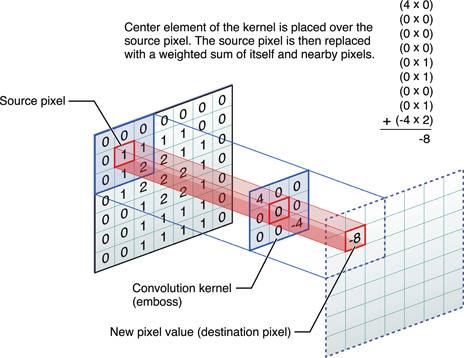
\includegraphics[width=0.8\textwidth]{convolutionFilter.jpg}
\end{figure}
Convolution neural networks are typically used for computer vision technologies,
as elements in an image are generally more related to each other if they are
closer to each other. However, as sound files are really just a large array of
air pressures, the frequency of the various tones are not known. Thus,
convolutional networks could be used to find patterns within the air pressures,
determine the frequency of different sections, and through that, determine the
,tone of the music at various points. Since music does have patterns in sounds
that are closer together to each other, this solution is valid.

\subsection{Autoencoder}
Autoencoders are also a form of unsupervised learning algorithm, as they simply
find a relationship within the data. They are useful as they can reduce the
dimensionality of the data, making the computations faster for the recurrent
neural network. An autoencoder is a two layer neural network, with the input
layer and desired output both being a sample from the input data. The weights
connecting the input to the hidden layer is generally referred to as the encoder
, and the weights connecting the hidden layer to the output layer is referred to
as the decoder. The hidden layer of the autoencoder is typically passed to more
unsupervised learning algorithms, or the primary model that is to be used.

\begin{figure}[H]
	\centering
	\caption{Simple autoencoder}
	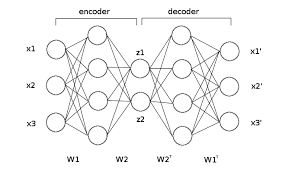
\includegraphics[width=0.7\textwidth]{autoencoderDiagram.jpg}
\end{figure}

The type of autoencoder used in this project will have sigmoid activation
functions, and be trained against mean squared error. The decoder part of the
model will utilize the identity for the activation function, being that no
nonlinearity will be applied to the activations.

\subsection{Rprop Trainer}
The training method that is used is RPROP, originally devised by Reidmiller and
Braun. This training method utilizes only the sign of the gradient, and has a
stored matrix representing the magnitude in which the algorithm will update the
parameters. The reason this method will be used, is because this algorithm is
not affected by the vanishing gradient problem, or the exploding gradient
problem, as the algorithm only worries about the sign of the gradient, being
positive or negative. Furthermore, the algorithm approaches the minimum for the
error function exponentially, as it will increase the magnitutde of the update
if the previous update was in the same direction as the current update. For
example, if the first update added 1 to a paramater, and the second gradient was
also positive, the second update would add 1 multiplied with some constant,
being 1.2 in this case. As a result, the updates can potentially increase
exponentially, and will find the gradient with less iterations. However, this
algorithm can only be used for batch learning, and as a result, could be slower.

\subsection{Back Propagation Through Time}
The gradient for a recurrent neural network differs significantly from a neural
network, in that it is dependent on all the data given to the network before it,
whereas the gradient for a neural network given a data sample, is that data
sample. This process of finding the gradient throughout the previous data
samples is known as back propagation through time, as to find the gradient, one
needs to back propagate through the previous data samples. Thus, if the data
sequence passed to a recurrent neural network is too long, then training the
model will take a large amount of time.

\subsection{Implementational Details}
Python and Theano are used to test these models. Theano is considered to be very
fast, amongst the machine learning community, which is why it is used. Also, a
gpu will be utilized to increase the performance of all models. The music
utilized for the model will have come from Youtube.

\section{Comparison}

\section{Data}

\section{Appendix}
\subsection{Code for Autoencoder}
%\lstinputlisting[language=Python]{DeepLearning.py}

\begin{thebibliography}{9}
	\bibitem{deepnetworktrainers}
		Larochelle, Hugo et al. ``Exploring Strategies for Training Deep Neural
		Networks.'' \textit{Journal of Machine Learning Research} (2009): n\. pag.
		Web. 10 May 2016.

	\bibitem{dnn dimensionality}
		Hinton, G.E. and Salakhutdinov, R. R. ``Reducing the Dimensionality of
		Data with Neural Networks.'' \textit{Science} (2006). 504--507. Web. 10
		May 2016

	\bibitem{unsupervised}
		Erhan, Dumitru et al. ``Why Does Unsupervised Pre-training Help Deep
		Learning?'' \textit{University of Montreal}:201--208. Web. 10 May 2016.

	\bibitem{rbm}
		Hinton, Geoffrey. ``A Practical Guide to Training Restricted Boltzmann
		Machines.'' \textit{University of Toronto (2010)}: 1--20. Web. 10 May
		2016.

	\bibitem{rbm intro}
		Fischer, Asja and Igel, Christian. ``An Introduction to Restricted
		Boltzmann Machines. \textit{University of Copenhagen (2012)}: 14--36. Web.
		10 May 2016.

	\bibitem{lstm}
		Horchreiter, Sepp and Schmidhuber, Jurgen. ``Long Short-Term Memory.''
		\textit{Technical University of Munich (1997)}: 1--32. Web. 10 May 2016.

	\bibitem{cw-rnn}
		Koutnik, Jan et al. ``A Clockwork RNN.'' \textit{Dalle Molle Institute
		for Artificial Intelligence Research}: n\. pag. Web. 25 May 2016.

\end{thebibliography}

\end{document}
